\documentclass[12pt]{report}
\usepackage{graphicx} % Required for inserting images
\linespread{1.2}

\usepackage[dvipsnames]{xcolor}
\usepackage{tikz}
\usepackage[breakable]{tcolorbox}
\usepackage{colortbl}
\appto{\bibsetup}{\raggedright}

\tikzstyle{mybox} = [draw=BrickRed, fill=BrickRed!5, ultra thick, rectangle, rounded corners, inner sep=10pt, inner ysep=15pt, text width=0.90\textwidth, align=left] 
\tikzstyle{boxtitle} = [fill=BrickRed, text=Apricot!20, ultra thick, rectangle, rounded corners, inner sep=10pt, inner ysep=8pt, text width=0.90\textwidth]

\newcommand{\BoxDef}[2]{%
\vspace*{10px}
\noindent

\begin{center}
\begin{tikzpicture}
    \node[mybox](box){\rule{0pt}{30pt}\ignorespaces#2\unskip};
    \node[boxtitle, anchor=north west] at (box.north west) {\textbf{#1}};
\end{tikzpicture}
\end{center}
}

\newcommand{\ceil}[1]{\left\lceil#1\right\rceil}

\usepackage[hidelinks]{hyperref}
\usepackage{amssymb}
\usepackage{amsmath}
\usepackage{bm}
\usepackage[top=2.5cm, bottom=2.5cm, left=3cm, right=3cm, centering]{geometry}
\usepackage{algorithm}
\usepackage{algpseudocode}
\usepackage{tabularx}
\usepackage{tabularray}

\begin{document}

\begin{titlepage}
\hrule
\vspace{15pt}
\begin{center}
    \Huge{\textbf{\Huge \textbf{Advanced Databases 23-24}} \\ Notes}\\
\end{center}
\vspace{15pt}
\hrule
\vfill
\hrule
\begin{center}
    \Large University of Pisa \\ M.Sc. in Computer Science
\end{center}
\end{titlepage}

\tableofcontents

\chapter{Introduction}

The most common use of information technology is to store and retrieve data, be it text, images, video, or audio files. As the amount of data generated by several processes increases as time goes on, storage systems must evolve to guarantee reliable access to the data, as well as fast and efficient retrieval. Data is typically stored into \textbf{databases} (\textbf{DBs}), which are housed in a permanent memory.

The technology on which permanent memory is based uses magnetic \textbf{disks}, containing a set of platters that rotate at relatively slow speeds (compared to CPU speed), which can be interacted with by using heads attached to moving arms. Each platter has on both surfaces a set of rings, called \textbf{tracks}, which, except for the innermost and outermost ones, are used to store information. Each track is subdivided into \textbf{sectors} of the same size, which correspond to the smallest unit of transfer allowed by the hardware. Typical sector sizes are 512 bytes, 1 KB, 2 KB, or 4 KB. There are from 500 to 1000 sectors per track, and about 100K tracks per surface of a single platter.

The \textbf{access time} needed to read a section of the disk is given by the seek time (needed to move the head), the rotational delay (given by the spinning of the disk itself), and the transfer time (needed to read/write the data). These operations take several milliseconds to be completed, which are definitely slower than any operation relative to the \textbf{main memory} (\textbf{RAM}), taking only a few nanoseconds in total. 

Despite this disparity, disks are still today the preferred technology to store data. Main memory is, in fact, volatile: once the machine stops receiving electricity powering it on, any information on the RAM is lost forever. On the other hand, disks provide reliable storage: the information written on them can be retrieved even if the machine is turned off and on. A newer technology, called \textbf{solid state storage}, and, in particular, \textbf{flash memory}, has risen in popularity in the last years. It provides the reliability of disks and much faster operations, although they still haven't become the new standard since they tend to be expensive.
\chapter{Overview of a DBMS}

This chapter will give a general overview of the structure of a centralized \textbf{DBMS} (\textbf{Data Base Management System}) based on the relational data model, describing its components and their respective functionalities.

\section{Architecture}

A database is a collection of homogeneous sets of data, with relationships defined among them, stored in permanent memory, and used via a DBMS.

\BoxDef{DBMS}{
A DBMS is a software that provides the following functionalities:
\begin{itemize}
    \item A language to describe the \textbf{schema} of the database (a collection of definitions that describe the data structures), restrictions on the allowed data types, and the relationships among data sets;
    \item The data structures for storage and efficient retrieval of large amounts of data;
    \item A language to guarantee secure access to the data only to authorized users;
    \item A \textbf{transactions} mechanism to protect data from HW/SW malfunctions and errors during concurrent access.
\end{itemize}
}

The architecture of a DBMS provides the following basic components:
\begin{itemize}
    \item The \textbf{Storage Engine}, which includes modules supporting:
    \begin{itemize}
        \item \textbf{Permanent Memory Manager};
        \item \textbf{Buffer Manager};
        \item \textbf{Storage Structures Manager};
        \item \textbf{Access Methods Manager};
        \item \textbf{Transaction and Recovery Manager};
        \item \textbf{Concurrency Manager}.
    \end{itemize}

    \item The \textbf{Relational Engine}, which includes modules supporting:
    \begin{itemize}
        \item \textbf{Data Definition Language};
        \item \textbf{Query Manager};
        \item \textbf{Catalog Manager}.
    \end{itemize}
\end{itemize}
In real systems the functionalities of these modules are not completely separated in different components (as in Figure \ref{fig:DBMS_schema}), but this overview can help in understanding the purpose of each of them. 

\begin{figure}[h]
    \centering
    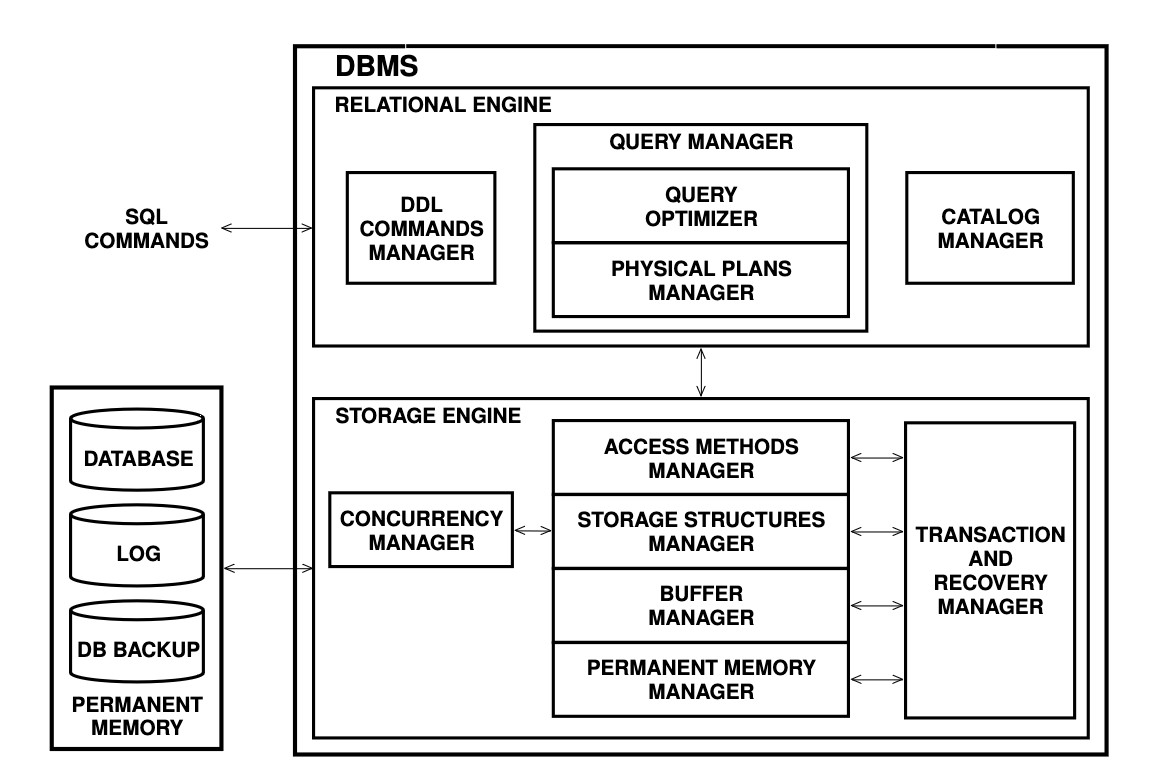
\includegraphics[width=0.75\linewidth]{img/DBMS schema.png}
    \caption{The architecture of a DBMS.}
    \label{fig:DBMS_schema}
\end{figure}

\subsection{Permanent Memory Manager}

The PMM manages page allocation and deallocation on disk storage. It hides the disk characteristics and the operating system, as it provides an abstraction of the memory as a a set of databases, each consisting of a set of logical files of \textbf{physical pages} (or blocks) of fixed size. The physical pages of a file are numbered consecutively starting from 0, and their number can grow dynamically with the only limitation being the available space in the permanent memory.

\nocite{*}
\bibliographystyle{plain}
\clearpage\bibliography{bibliography}

\end{document}
